% Created 2021-03-04 jue 10:29
% Intended LaTeX compiler: pdflatex
\documentclass[presentation,aspectratio=169]{beamer}
\usepackage[utf8]{inputenc}
\usepackage[T1]{fontenc}
\usepackage{graphicx}
\usepackage{grffile}
\usepackage{longtable}
\usepackage{wrapfig}
\usepackage{rotating}
\usepackage[normalem]{ulem}
\usepackage{amsmath}
\usepackage{textcomp}
\usepackage{amssymb}
\usepackage{capt-of}
\usepackage{hyperref}
\usepackage{khpreamble}
\usepackage{amssymb}
\usepgfplotslibrary{groupplots}
\newcommand*{\shift}{\operatorname{q}}
\DeclareMathSymbol{\Omega}{\mathalpha}{letters}{"0A}% italics
\DeclareMathSymbol{\varOmega}{\mathalpha}{operators}{"0A}% upright
\providecommand*{\upOmega}{\varOmega}% for siunitx
\usepackage[binary-units=true]{siunitx}
\usepackage{circuitikz}
\usetheme{default}
\author{Kjartan Halvorsen}
\date{2021-03-04}
\title{El motor electrico de corriente continua}
\hypersetup{
 pdfauthor={Kjartan Halvorsen},
 pdftitle={El motor electrico de corriente continua},
 pdfkeywords={},
 pdfsubject={},
 pdfcreator={Emacs 26.3 (Org mode 9.4.4)}, 
 pdflang={English}}
\begin{document}

\maketitle

\section{El motor electrico de corriente continua}
\label{sec:org5f4cd9a}
\begin{frame}[label={sec:org058fce4}]{Fuerza en un conductor eléctrico en un campo magnético}
\begin{center}
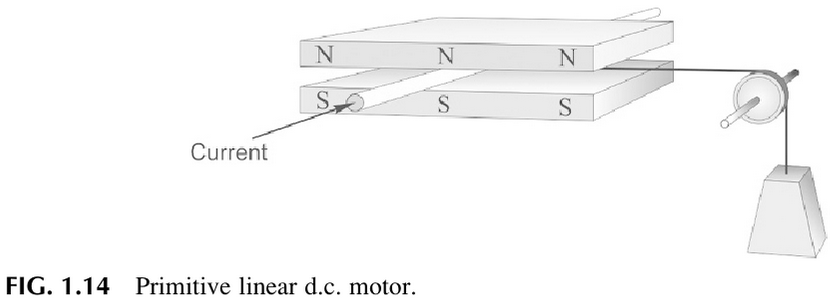
\includegraphics[width=0.4\linewidth]{../../figures/HD-fig1_14.png}
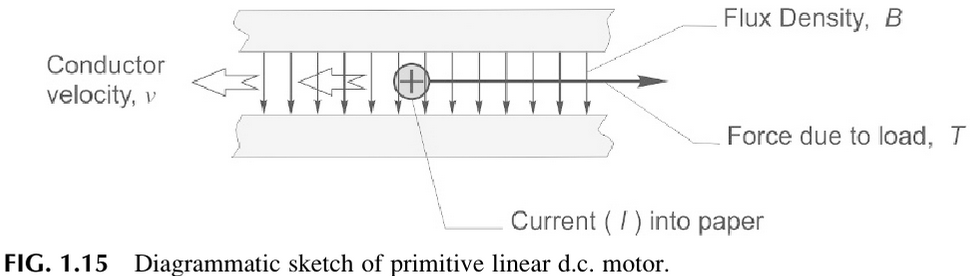
\includegraphics[width=0.53\linewidth]{../../figures/HD-fig1_15.png}
\end{center}

La fuerza electromagnética en el conductor es \alert{proporcional a la corriente}:
\[F=k_mI=(Bl_m)I,\] donde \(B\) es la densidad del flujo magnético en el entrehierro, \(I\) es la corriente, y \(l_m\) es la longitud del cable. Se junta varias cables en una bobina para aumentar la fuerza.
\end{frame}

\begin{frame}[label={sec:org5fc7843}]{Rotación}
\begin{center}
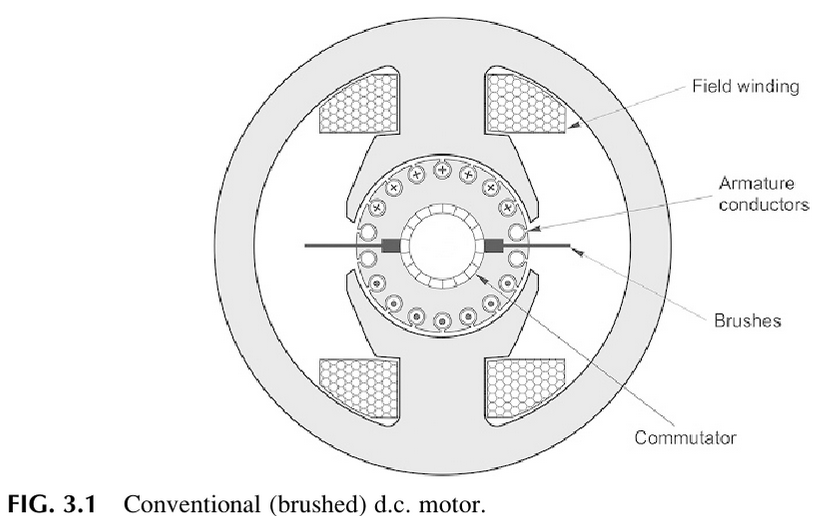
\includegraphics[width=0.4\linewidth]{../../figures/HD-fig3_1.png}
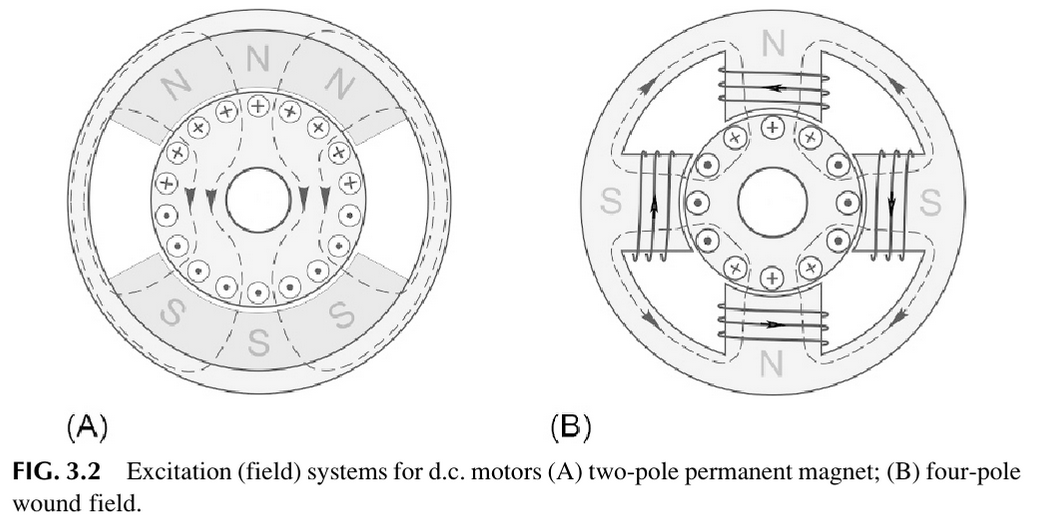
\includegraphics[width=0.53\linewidth]{../../figures/HD-fig3_2.png}
{\footnotesize Fuente: Hughes and Drury}
\end{center}
\end{frame}

\begin{frame}[label={sec:org5b31436}]{Las dos ecuaciónes del motor eléctrica CC}
\begin{block}{Fuerza generado en el conductor por la corriente en el campo magnético}
\[ F(t) = k_m i(t) \quad\Leftrightarrow\quad T(t) = k_m r i(t),\]
dónde \(r\) es el radie del motor.
\end{block}

\begin{block}{Voltaje generado por el movimiento del conductor en el campo magnético}
\[ e(t) = k_v v(t) \quad\Leftrightarrow\quad e(t) = k_v r \omega(t)\]
\(e(t)\) se llama \emph{Fuerza contraelectromotriz} o \emph{Back electro-motive force (Back e.m.f.)} en inglés.
\end{block}
\end{frame}
\begin{frame}[label={sec:orgf3bc971}]{Circuito equivalente}
Motor CC con excitación separada
\begin{center}
  \begin{circuitikz}
    \draw (4,1) node[elmech](motor){M};
    \draw (motor.north) to[R=$R$] (4,4) to[L=$L$] (0,4)
    to[american voltage source, label=$V$] (0,0) -| (motor.south);
    \draw[thick,->>](motor.right)--++(1,0)node[midway,above]{$\omega$};

    \node[] at (2, -0.8 cm) {\(L \frac{d}{dt}i(t) +  Ri(t) + k\omega(t) = V\)};

    \node[] at (2, 4.5 cm) {Armadura};

    \begin{scope}[xshift=8cm]
    \draw (0,1) to (4,1) to[R=$R_f$] (4,3) to[L=$L_f$] (0,3)
    to[american voltage source, label=$V_f$] (0,1);
    \node[] at (2, 4.5 cm) {Campo};
    \end{scope}
  \end{circuitikz}
\end{center}

\begin{center}
Newton: \(J\frac{d}{dt}\omega(t) = ki(t) - T_l(t)\)
\end{center}
\end{frame}


\begin{frame}[label={sec:org0ae304c}]{Velocidad con carga constante}
\begin{align}
L\frac{d}{dt}i(t) + Ri(t) + k\omega(t) &= V(t)\\
J\frac{d}{dt}\omega(t) &= ki(t) - T_l(t)
\end{align}

En estado estable: \(i(t) = I\), \(\omega(t) = \omega\).

\begin{align}
0 + RI + k\omega &= V\\
0 &= kI - T_l
\end{align}

\[\omega = f(V, T_l) = \frac{V}{k} - \frac{RI}{k} = \frac{V}{k} - \frac{RT_l}{k^2}\]
\end{frame}

\begin{frame}[label={sec:orgabf534f}]{Velocidad con carga constante}
\[\omega = f(V, T_l) = \frac{V}{k} - \frac{RT_l}{k^2}\]
Un motor especifico tiene el constante \(k=\unit{4}{\newton\meter\per\ampere}\) y resistencia \(R=\SI{0.2}{\ohm}\). Se aplica un voltaje de \(V=\unit{100}{\volt}\) sobre su armadura.


\alert{Actividad individual} Dibuje como la velocidad en estado estable depende de la carga \(T_l\). ¿Cuál es el par de parada?

\begin{center}
  \begin{tikzpicture}[xscale=0.8]
    \draw[->] (0, 0) -- (9, 0) node[right] {$T_l$ [\unit{}{\newton\meter}]};
    \draw[->] (0, 0) -- (0, 3) node[left] {$\omega$};
    \foreach \t in { 1, 2, ..., 8} {
    \draw (\t, 0) -- (\t, -0.1) node[below] {\t{}00};
    }
    \end{tikzpicture}

\end{center}
\end{frame}

\begin{frame}[label={sec:org0cd05e1}]{Velocidad con carga constante}
\[\omega = f(V, T_l) = \frac{V}{k} - \frac{RT_l}{k^2}\]

\begin{center}
   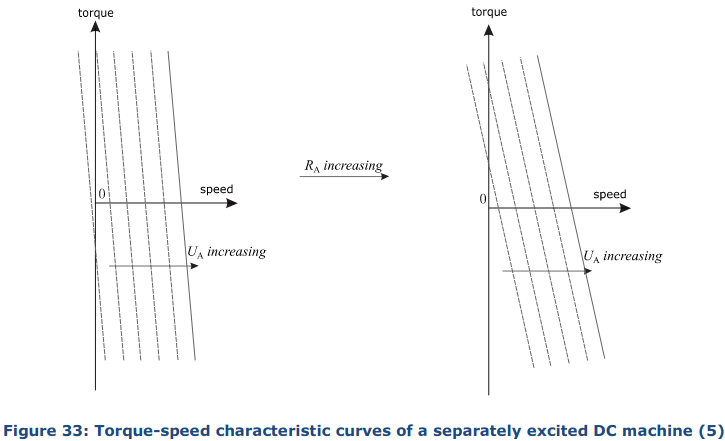
\includegraphics[width=0.6\linewidth]{../../figures/infineon-motor-handbook-fig33.png}\\
   {\footnotesize Fuente: Infineon: Motor handbook}
   \end{center}
\end{frame}

\begin{frame}[label={sec:orgbf75bbc}]{Arranque}
Para un motor parada, la fuerza contraelectromotriz es cero, y solo la resistencia y la inductancia de la armadura limiten la corriente.

\begin{center}
  \begin{circuitikz}
    \draw (4,1) node[elmech](motor){M};
    \draw (motor.north) to[R=$R$] (4,4) to[L=$L$] (0,4)
    to[american voltage source, label=$V$] (0,0) -| (motor.south);
    \draw[thick,->>](motor.right)--++(1,0)node[midway,above]{$\omega$};

    \node[] at (2, -0.8 cm) {\(L \frac{d}{dt}i(t) +  Ri(t) + k\omega(t) = V\)};
  \end{circuitikz}
\end{center}


Hay que tener cuidado en el arranque para que la corriente no sube a niveles excedentes. \alert{Solución} control de la corriente por retroalimentación.
\end{frame}

\section{Modeling}
\label{sec:orge867788}
\begin{frame}[label={sec:orgb269181}]{Modelo de bloques del circuito equivalente}
\begin{center}
  \begin{circuitikz}[yscale = 0.5]
    \draw (4,2) node[elmech](motor){M};
    \draw (motor.north) to[short] (4,4) to[R=$R$] (2,4) to[L=$L$] (0,4)
    to[american voltage source, label=$V$] (0,0) -| (motor.south);
    \draw[thick,->>](motor.right)--++(1,0)node[midway,above]{$\omega$};

    \node[] at (9, 4 cm) {\(L \frac{d}{dt}i(t) +  Ri(t) + k\omega(t) = V\)};
    \node[] at (9, 2 cm) {\(\frac{d}{dt}i(t) = \frac{1}{L} \Big(-Ri(t) - k\omega(t) + V\Big)\)};
    \end{circuitikz}
    \end{center}
    \begin{center}
    \begin{circuitikz}[yscale = 1]
  \begin{scope}[xshift=8cm, yshift=-1cm,
  block/.style={rectangle, draw, minimum width=12mm, minimum height=10mm},
  amp/.style = {regular polygon, regular polygon sides=3,
        draw, fill=white, text width=1em,
        inner sep=1pt, outer sep=0mm,
        shape border rotate=-90},
	summ/.style = {circle, draw, inner sep = 1pt},]
   \node[block,] (int) at (0,0) {$\int$};
   \node[amp, left of=int, node distance=30mm] (oneoverL) {$\frac{1}{L}$}; 
   \draw[->] (oneoverL) -- node[above] {$\frac{d}{dt}i(t)$} (int);
   \node[summ, left of=oneoverL, node distance=20mm] (sum) {\small $\Sigma$};
   \node[coordinate, left of=sum, node distance=35mm] (Vin) {};
   \draw[->] (Vin) -- node[above, very near start] {$V$} node[coordinate, pos=0.6] (mp) {} (sum);
   \node[amp, above of=mp, node distance=15mm] (mkonst) {$-k$};
   \draw[->] (int) -- node[above, near end] {$i(t)$} ++(25mm, 0);
   \draw[->] (mkonst) ++(-2cm, 0) -- node[above, near start] {$\omega(t)$} (mkonst);
   \draw[->] (mkonst) -| (sum);
   \draw[->] (sum) -- (oneoverL);
   \node[amp, below of =int, node distance=16mm, rotate=180, white] (fb) {\rotatebox{-180}{$-R$}};

   \end{scope}
  \end{circuitikz}
  \end{center}

\alert{Actividad en pares} Completa el diagrama.
\end{frame}






\begin{frame}[label={sec:org2bfa6c7}]{Transmisión}
\end{frame}

\begin{frame}[label={sec:org7c4db74}]{Transmisión}
  \begin{center}
  \begin{circuitikz}[xscale = 0.8]
\begin{scope}[xshift=8cm, yshift=-1cm,
block/.style={rectangle, draw, minimum width=12mm, minimum height=10mm},
amp/.style = {regular polygon, regular polygon sides=3,
      draw, fill=white, text width=1em,
      inner sep=1pt, outer sep=0mm,
      shape border rotate=-90},
      summ/.style = {circle, draw, inner sep = 1pt},]
 \node[block,] (int) at (0,0) {$\int$};
 \node[amp, left of=int, node distance=25mm] (oneoverL) {$\frac{1}{L}$}; 
 \draw[->] (oneoverL) -- node[above] {$\frac{d}{dt}i$} (int);
 \node[summ, left of=oneoverL, node distance=15mm] (sum) {\small $\Sigma$};
 \node[coordinate, left of=sum, node distance=45mm] (Vin) {};
 \draw[->] (Vin) -- node[above, very near start] {$V$} node[coordinate, pos=0.8] (mp) {} (sum);
 \node[amp, above of=mp, node distance=15mm] (mkonst) {$-k$};
 \node[amp, left of=mkonst, node distance=20mm] (gr) {$g_r$};
 \node[amp, right of=int, node distance=25mm] (mk2) {$k$};
 \node[amp, right of=mk2, node distance=20mm] (gr2) {$g_r$};
 \draw[->] (int) -- node[coordinate, pos=0.5] (meas) {} node[above] {$i$} (mk2);
 \draw[->] (mk2) -- node[above] {$T_m$} (gr2);
 \draw[->] (gr2) -- node[above] {$T_e$} ++(15mm, 0);
 \draw[->] (gr) ++(-2cm, 0) -- node[above, near start] {$\omega_e$} (gr);
 \draw[->] (gr) -- node[above, ] {$\omega_m$} (mkonst);
 \draw[->] (mkonst) -| (sum);
 \draw[->] (sum) -- (oneoverL);
 \node[amp, below of =int, node distance=16mm, rotate=180] (fb) {\rotatebox{-180}{$-R$}};
 \draw[->] (meas) |- (fb);
 \draw[->] (fb) -| (sum);
 \end{scope}
\end{circuitikz}
\end{center}

Para transmisión (\(\omega_m = g_r\omega_e\)) perfecta:
\[\underbrace{T_m\omega_m}_{\text{potencia que entra}} = \underbrace{T_e\omega_e}_{\text{potencia que sale}}\]
\end{frame}
\end{document}